\documentclass[12pt,twoside]{article}

\usepackage{float}
\usepackage{amsmath}
\usepackage{tikz}

\usetikzlibrary{arrows.meta}

\begin{document}
\title{AP Physics C: The Tortoise and the Hare Lab}
\author{Raja Williams}
\date{September 2023}
\maketitle

\section{Objective}
The Tortoise and the Hare Lab seeked to predict, test and determine the meeting
point of two constant velocity buggies when both start moving towards each
other, or toward the same point. Two buggies were assigned to each group, as
well as two lines on the floor to denote starting locations for the buggies and
for predicting the meeting point. One of these buggies is around twice the speed
of the other.

\section{Procedure}

\begin{enumerate}
\item Measure the distance between the assigned lines.
\item Utilizing a meter stick, measure the amount of time it takes each buggy to
    go 1 meter using a stopwatch, specifically paying attention to the front
    wheel of the buggy. A diagram is visible in Figure \ref{fig:step2}.
\begin{figure}[h]
    \centering
    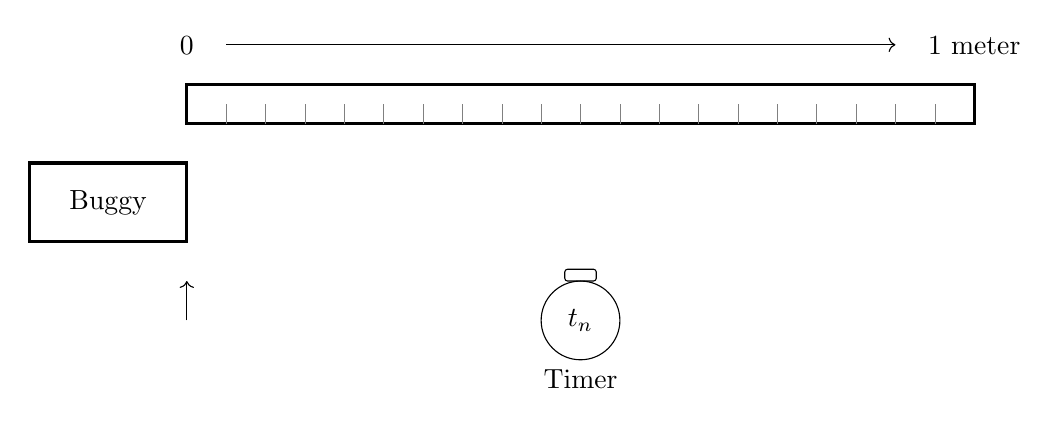
\begin{tikzpicture}
        \draw[very thick] (0,0) rectangle (-2,1);
        \draw[very thick] (0,1.5) rectangle (10, 2);
        \draw[->] (0, -1) -- (0, -0.5);       
        \draw (-1, 0.5) node {Buggy};
        \draw (0, 2.25) node[anchor=south] {0};
        \draw[->] (0.5, 2.5) -- (9, 2.5);       
        \draw (10, 2.25) node[anchor=south] {1 meter};
        \draw[rounded corners=1] (4.8,-0.35) rectangle (5.2, -0.5);
        \draw (5, -1) circle [radius=0.5];
        \draw (5, -1) node {$t_n$};
        \draw (5, -1.75) node {Timer};
        \foreach \x in {0.5,1,...,9.5}
            \draw[gray, very thin] (\x,1.5) -- (\x,1.75);
    \end{tikzpicture}
    \caption{Abstract diagram of Step 2 setup.}
    \label{fig:step2}
\end{figure}
\item To predict the meeting point of the two buggies, solve a system of
    equations utilizing the distance measured in Step 1 and calculated speeds
    from Step 2. Lay down a piece of tape on the floor at the predicted meeting
    point.
\item Then, set both buggies off side by side to test the predictions from Step
    3. A video with a timer visible in frame should be recorded for later
    reference of timing. Use the tape to see if prediction is correct.

\end{enumerate}

\section{Observations and Data}

We were assigned Lines 6 and 8, with both buggies going the same direction. The
distance measured between Lines 6 and 8 was 112 cm or 1.12 meters.

We received Buggy D and Buggy M, designated Buggy 1 and Buggy 2 respectively.

\begin{figure}[H]
    \centering
    \begin{tabular}{| l l l |}
        \hline
        Buggy & Trial & Travel Time (1 m) \\ \hline
        Buggy 1 & Trial 1 & 5.13 seconds \\
                & Trial 2 & 5.38 seconds \\
                & Trial 3 & 5.21 seconds \\ \hline
        Buggy 2 & Trial 1 & 2.85 seconds \\
                & Trial 2 & 2.84 seconds \\
                & Trial 3 & 2.82 seconds \\
        \hline
    \end{tabular}
    \caption{Buggy Travel Time by Trial}
\end{figure}

When the buggies were tested, both reached the same position at $T+5.71$ seconds,
where $T$ is the time at which the buggies started moving. The predicted meeting
point was clearly off by several buggy lengths.

\section{Analysis}

First, the times from each buggy and their trials were averaged. Final
calculations visible in Figure \ref{fig:average}.

\begin{figure}[h]
    \centering
    \begin{tabular}{| l l l |}
        \hline
        Buggy & $\bar{t}$ & $\text{1 m}/\bar{t}$ \\ \hline
        Buggy 1 & 5.24 seconds & 0.191 m/s \\
        Buggy 2 & 2.84 seconds & 0.352 m/s \\
        \hline
    \end{tabular}
    \caption{Buggy Average Travel Time and cart speed}
    \label{fig:average}
\end{figure}

The speed of each buggy can be calculated by using
\begin{equation}
    \frac{\text{1 meter} }{\bar{t} \text{ seconds}} \quad m/s
\end{equation}
where $\bar{t}$ is the average of amount of seconds measured for one buggy.
Final calculations for $\bar{t}$ is visible in Figure \ref{fig:average}.

There is some uncertainty in the measurements given due to human reaction time
of the person holding the timer. We converted measurements and calculations to
cm and cm/s at this point, as most were under 1 m and/or m/s. Then, we solved
the system of equations given in equation \ref{eq:system}.

\begin{align}
    \begin{split}
        x_P &= 19.1 \text{ cm/s} \cdot t_P + 112 \text{ cm} \\
        x_P &= 35.2 \text{ cm/s} \cdot t_P
        \label{eq:system}
    \end{split}
\end{align}

Solving for $t_P$,

\begin{align}
    \begin{split}
        35.2 \text{ cm/s} \cdot t_P &= 19.1 \text{ cm/s} \cdot t_P + 112 \text{ cm} \\
        16.2 \text{ cm/s} \cdot t_P &= 112 \text{ cm} \\
        t_P &= 6.91 \text{ seconds}
    \end{split}
    \label{eq:expected}
\end{align}

This means that the buggies will meet at a predicted $T+6.91$ seconds, where $T$ is
the time at which the buggies both start moving. To find the distance at which
the buggies meet, the $t_P$ value computed was plugged in to equation \ref{eq:system}.

\begin{align}
    \begin{split}
        x_P &= 35.2 \text{ cm/s} \cdot t_P \\
        x_P &= 35.2 \text{ cm/s} \cdot 6.91 \text{ seconds} \\
        x_P &= 243.23 \text{ cm}
    \end{split}
\end{align}

When the buggies were tested against each other, the predicted $t_P$ from
equation \ref{eq:expected} was 1.2 seconds more than the actual result of $t_E =
5.71 \text{ seconds}$. It is unclear what $x_E$ is from the recorded video.

\section{Conclusion}

The primary source of error can be attributed to human error of the operator
holding the timer in Step 2. The reaction time of the operator as well as the
imprecision of trying to measure the timing at a vague point (where the front
wheel meets the end of the meter stick) made our predicted values $t_P$ and
$x_P$ very imprecise.

In the end, our group was not able to determine the actual meeting point $x_E$,
at least to a precision of less than multiple tens of centimeters.

\end{document}
